\clearpage
\section{Veřejné statky (definice, rozhodování o veřejných statcích, úhrada za veřejný statek).}
\subsection{Definice}
\begin{itemize}
    \item Nejsou vyloučitelné ve spotřebě (vyloučitelnost ve spotřebě: spotřeba jedním člověkem nemá vliv 
    na užitek jiných lidí, např.: někdo vypije litr mléka), (nelze pouliční osvětlení zapnout jen pro někoho)
    \item Nejsou zmenšitelné ve spotřebě (zmenšitelnost ve spotřebě - nabízené množství je konečné číslo, je omezené)
    \item Čistě veřejné statky jsou nevylučitelné a nezmenšitelné ve spotřebě
    \item Jsou náklady na vytvoření statku, ale na poskytnutí už vytvořeného statku více lidem, jsou náklady nulové
    \item Mnoho je poskytováno vládou/státem z důvodů:
    \begin{enumerate}
        \item Soukromé společnosti by dosahovaly ztrát, protože poskytování statků vyžaduje náklady,
        za které nemůžou platit spotřebitelé, protože by se nejspíše našli \uv{černí pasažéři}, kteří by neplatili
        \item Nelze jej efektivně platit spotřebiteli, protože je nezmenšitelný a mezní náklady na uspokojení dalšího
        zákazníka jsou nulové
    \end{enumerate}
    \item Více typů statků:
    
    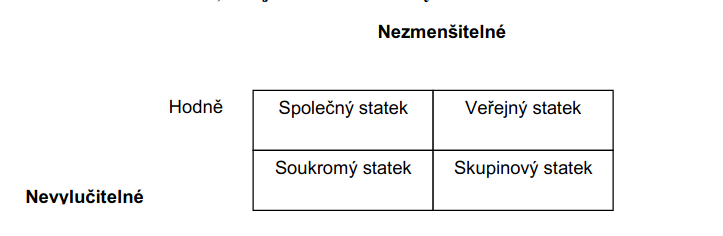
\includegraphics[width=15.5cm]{images/23_statky.png}
    
    \item společný: zmenšitelný, nevylučitelný; např. ryby v oceánu
    \item soukromý: zmenšitelný, vyloučitelný; zaplatím za něj, dostanu jej, např. mléko
    \item skupinový: nezmenšitelný, vyloučitelný; např. satelitní televize
\end{itemize}

\subsection{Rozhodování o veřejných statcích}
\begin{itemize}
    \item Stát nemusí zajišťovat vše, co je veřejný statek
    \item Prospěch by měl převýšit náklady (explicitní i implicitní), jinak je lepší se bez něj obejít (městský ohňostroj)
    \item Prospěch lze určovat dotázáním lidí, kolik by za statek byli ochotni zaplatit, součet těchto částek 
    (u soukromých statků je to maximální hodnota, kterou by jednotlivý zákazník byl ochoten zaplatit)
    \item Zajištění státem má také smysl, pouze pokud neexistuje levnější způsob, jak to udělat
    \item O množství nerozhodují spotřebitelé, ale vláda/stát/obec, spotřebitelé nemohou vyjádřit své preference,
    proto neexistuje mezní užitek veřejného statku
    \item Rozhoduje se v politickém procesu, prostřednictvím voličů, tzv. \uv{veřejná volba}, politici se nemohou opřít
    o poptávku, protože neexistuje a nelze ji odhadnout
    \item Teorie veřejné volby
    \begin{itemize}
        \item vlády se chovají tak, aby získávaly co nejvíce hlasů
        \item po volbách: restriktivní politika (pokles inflace, růst nezaměstnanosti)
        \item před volbami: expanzivní politika (růst inflace, pokles nezaměstnanosti) - tento a předchozí bod: politické
        cykly
        \item Konkurence mezi politickými stranami, mohou měnit důchody voličů využíváním zásob kapitálu a práce
    \end{itemize}
\end{itemize}

\subsection{Úhrada za veřejný statek}
\begin{itemize}
    \item Různí lidé mají z veřejných statků různý užitek, ale stát nemá šanci tyto informace zjistit a nelze tedy
    vyměřit přesné daně z užitku
    \item Používá se:
    \begin{itemize}
        \item daň z hlavy - každý platí stejně
        \item regresivní daň - s růstem příjmů poměrově klesá
        \item proporcionální daň z příjmu - stejná relativní část příjmů
        \item progresivní daň - s růstem příjmů roste relativní daňové zatížení
    \end{itemize}
    \item Veřejné statky se poskytují všem ve stejném množství a ve stejné kvalitě
    \item Téměř všechny státy mají progresivní daňový systém
    \item Může se to zdát nespravedlivé k bohatým, jenže pokud by se zavedla proporcionální nebo fixní daň, omezovaly by 
    se statky, které mají pro bohaté největší cenu (parky, rekreace, čistý vzduch, veřejná bezpečnost, dobré silnice)
    \item Veřejné statky může stát nakupovat od soukromých firem, financuje z rozpočtu, tedy z daní
\end{itemize}
